\chapter{System Implementation}
\label{cha:system_implementation}
\quad Continual Learning is the application of a system capable of self-adjustment and able to learn from incoming data streams. The main competence of this system is indeed the ability to modify weights and biases to learn from the environment and continue to be accurate and reliable for the application. This thesis developed an easier CL system that has to replace a class with another one. In particular the Mnist \cite{deng2012mnist} class 0 will be replaced with a letter from the Emnist \cite{cohen2017emnist} dataset.

\section{Creation of the project}
\label{sec:creation_of_project}
\quad To modify weights and biases it is necessary to know how those values are structured and used. The CNN accelerator uses biases and weights after they are uploaded to memory, which is performed by functions automatically generated with the Software Development Kit (SDK) \cite{SDK}. This series of tools help the developers in many ways. The workflow consists of the first creation and training of a Neural Network model made by specific layers \cite{ai8x-training}. 
Afterward is the synthesis of the model \cite{ai8x-synthesis} , which creates C code that programs the MAX78000 for embedded execution. The program that synthesizes the model needs three inputs a quantized checkpoint file that holds the network weights, a YAML description of the network, and a numpy pickle file with sample input. The code generated by the synthesizer contains a log file that has valuable information about the Networks, which are the kernel map and the values used by each layer divided by processors. The kernel map is a chart 64x768 that shows which kernels are used by each layer. This work focuses on the last layer which uses the first 12 kernels. Furthermore, the layer values are written in layer order, the first row of each processor corresponds to the first output, and so on. These values correspond to the values of the kernel.

\section{Weights allocation}
\label{sec:weights_allocation}
\quad A kernel map is a useful tool needed to understand the order in which each weight is loaded in the memory and then convolute with the output from previous layers. To figure out the sequence of values is fundamental to compare the kernel file and the log file, in particular, each layer and processor with the correspondent kernel. Foremost, upon careful analysis, it is possible to notice that the Kernels are split into 12 portions. At the same time, in the log file, it is possible to observe that the processors are 12 and they are broken up into 10 channels (output neurons). Since there are 12 processors with 10 channels individually and 12 Kernels, it can be inferred that:

\begin{gather*}
    Kernel_j = \sum_{i=0}^{n}\sum_{j=0}^{m} Channel_{i,j}
\end{gather*}

\quad Where $n$ is the number of channels, $i$ is the $i$-$th$ channel, $m$ is the number of processors, and $j$ is the $j$-$th$ processor. 
Each channel piece represents the values of the weights related to their kernel, as seen in figure \ref{weights_allocation}. The bottom line is that every first channel of each processor corresponds to the first output class, the second channel to the second output class, and so forth. 

\begin{figure}[!ht]
\centerline{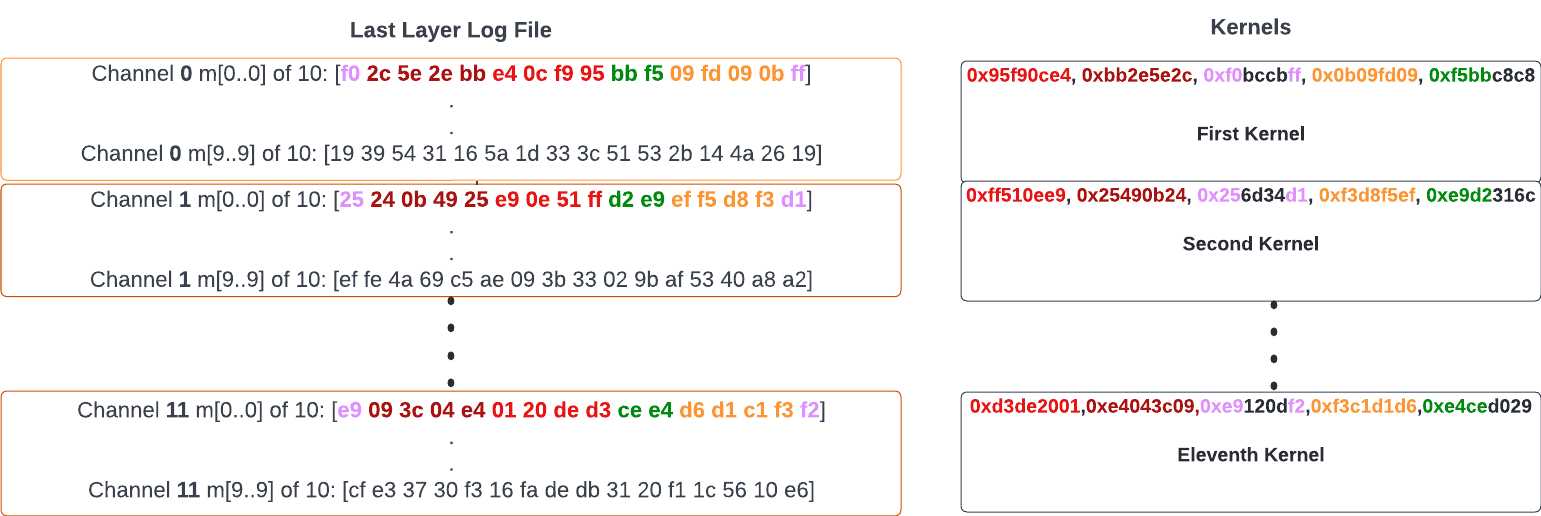
\psfig{file=Images/channel_weigths.png,width=0.9\textwidth}}
\caption{Channels of the last layer together with their correspondent place in the Kernels array}
\label{weights_allocation}
\end{figure}

\section{Last Layer Operation}
\label{sec:last_layer_operation}
\quad Continual Learning bases its functionality on weights update. To perform this operation it is necessary to know the network output with some input. So the first update happens after a complete inference. Since inferences take place inside the hardware-based accelerator, the only way to find out the output of each channel is to multiply the last but one layer output from the CNN accelerator by the weights of channels. This operation is needed because it's hard to find the single output of each channel directly inside the accelerator memory. A solution is to load each layer in succession in the memory, stop the inference at the penultimate layer and unload the result of it. The unload operation consists of a copy of values from specific memory areas. In this case study, the output of the frozen layer is flattened, and thanks to it and the weights from each channel, now it is possible to find the predictions needed for the update. The following chapters will discuss the implementation of the CL system. 

\begin{figure}[!ht]
\centerline{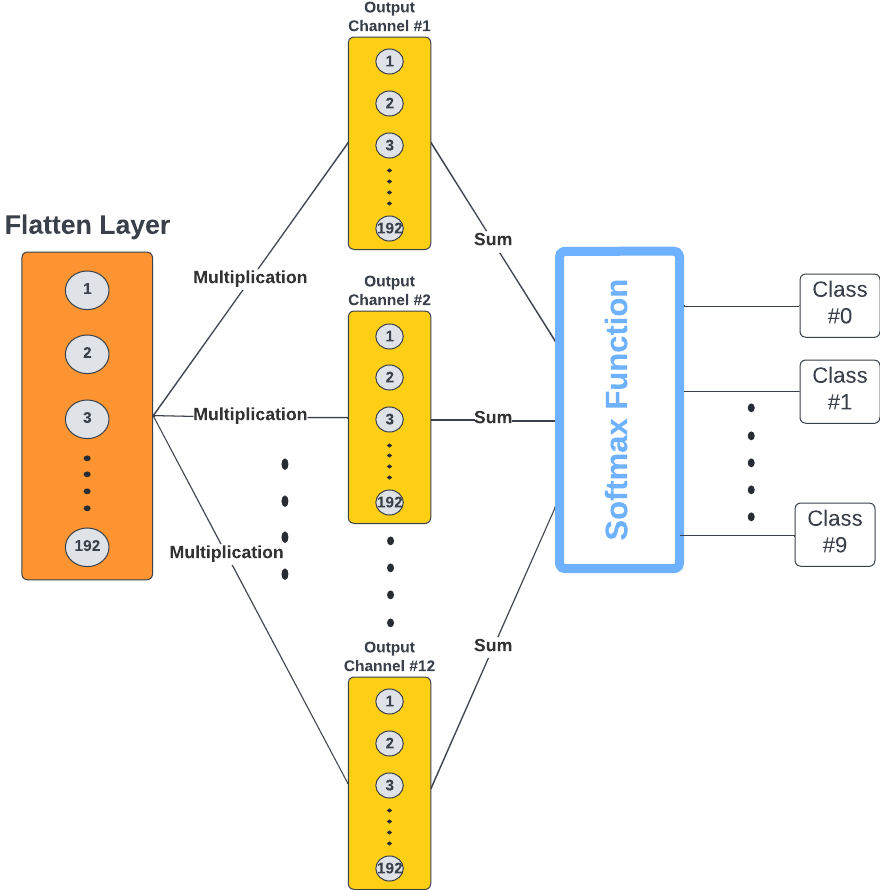
\psfig{file=Images/last_layer_weights_multiplication.png,width=0.6\textwidth}}
\caption{Flattened Layer multiplied by each kernels of last layer and then passed to Softmax Function to obtain percentage of each class}
\label{last_layer_per_weights}
\end{figure}

\section{Continual Learning System}
\label{cha:cl_system}
\quad Continual Learning (CL) is the application of real-time training to generate self-adjusting systems that can learn from never-seen Data. As mentioned in \autoref{sec:CL}, the main feature of CL is the ability of ML models to modify weights and biases to adapt to the environment and be accurate and longstanding reliable. However, CL models on MCU are a new idea that has been barely exploited in recent years. CL applications are not new to the ML scenery, but their function on tiny devices is a new approach. In this thesis, it is developed a similar CL system to the one proposed in \cite{Comprarison_of_Continual_learning_algorithm}. The paper analyses a comparison between different CL algorithm strategies regarding image classification and gesture recognition. The goal is to use a NN model to recognize letters written in the air through data recorded by an accelerometer sensor. The CL strategy is applied only to the last layer of the model, which is added to the pre-trained model and is trained every time a new sample is received.
The idea developed in this thesis started from the implementation of a similar system. The system allows a CNN model to perform continual learning, specifically for classification problems. In this implementation, the CL system is connected to the last layer, which substitutes one class with a not known one. The following section will explain the essential pipeline, and the implemented algorithm.
 
\section{Main pipeline of CL system}
\label{sec:main_pipeline}
\quad TinyML applications are built to be efficient and fast. To apply CL training on embedded devices, it is necessary to develop from scratch a framework that permits the implementation of the CL strategy. The framework is built around the Mnist project template using the same network and the same weights. The system involves the last layer of the network. It aims to enhance the classification abilities of the model, allowing the fine-tune and update of the classification weights and biases, which, over time, lead to better-performing models. The system is a supervised learning application. At every training step, the image fed to the system is class-known. In particular, this study replaces the digit 0 class with the letter A. 
\quad The basic idea of the developed system is to refresh and update the weights every time a new sample is received. This operation can be performed by implementing the standard ML training strategy, which consists of computing the prediction error and propagating it back to the weights. The update to apply depends directly on the impact the specific weights and biases have on the prediction outcome. Once this knowledge is available, it is possible to compute a feedback rule that allows finding the weights that better optimes the loss function. This study applies a CL application to a classification problem. Typically CNN models apply a Softmax activation function to the results of the classifications. This function is fundamental in this system because it permits obtaining a distribution of percentages. The application of CL in this project wants to train only the last layer, as seen in\ref{CL_pipeline}. The part of the model before the last layer is a black box, also called Frozen Model, which works the same for every inference and input. The update rule requires the Softmax function, the output of the Frozen model, the error between prediction and label, and the loss function. To better understand the update function, see \cite[p.~32]{Comprarison_of_Continual_learning_algorithm}

\begin{figure}[!ht]
\centerline{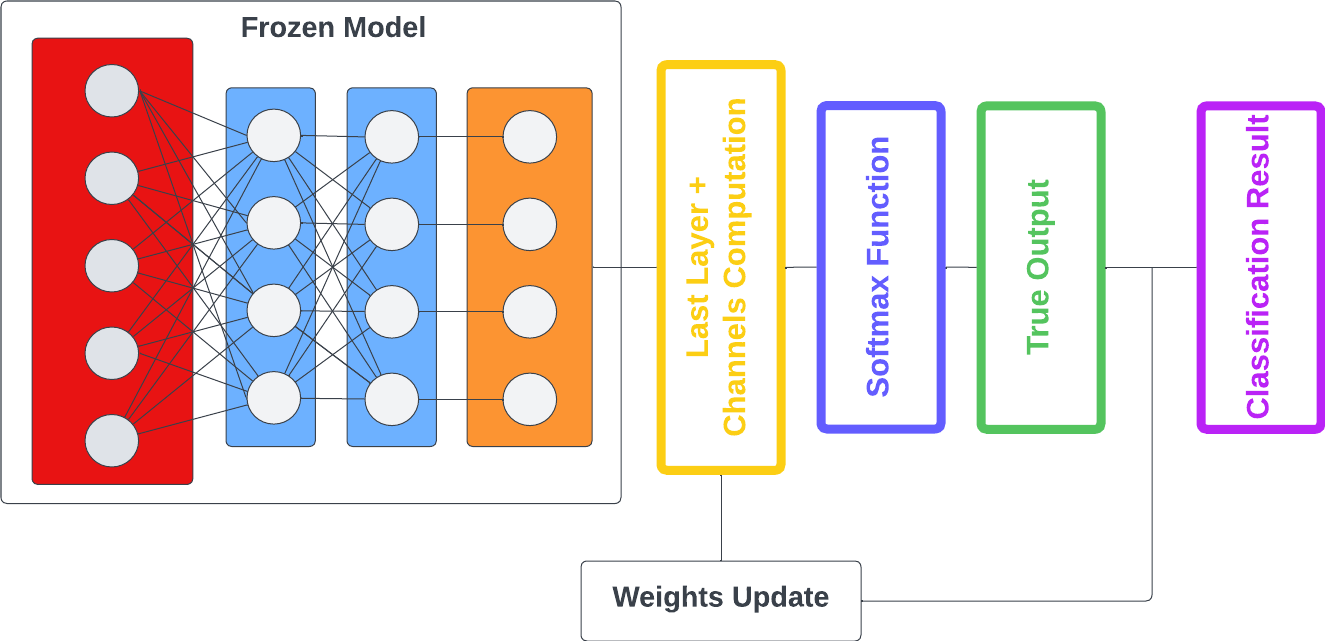
\psfig{file=Images/CL_pipeline.png,width=0.8\textwidth}}
\caption{Basic pipeline of Continual Learning application}
\label{CL_pipeline}
\end{figure}


\section{Implemented algorithm}
\label{sec:ol_alg}

\quad The study implements the TinyOL strategy for performing CL. The TinyOL algorithm is suitable for MCUs thanks to its ease of implementation and management of memories, which is a decisive constraint on embedded devices. The strategy follows the essential ML training step, which consists of computing the error from prediction and propagating it on the weights and biases through stochastic gradients descends (SGD). Its implementation consists of for loops for updating biases and the weights \cite{TinyOl_Paper}. As mentioned in \autoref{sec:weights_allocation}, the key elements that make the implementation complicated, are establishing the allocation of the weights and the rules used by the accelerator to work with them. Initially, the project only updated the weights of the first channel, and by reason of this, slowly, the weights allocation became coherent. Once understood the distribution, the implementation of the strategy could be done. The weights update rule for the TinyOL algorithm are: 


\begin{gather*}
   w_{i,j} = w_{i,j} - \alpha \cdot (y_i - t_i) \cdot x_{i,j} \\
   b_i = b_i - \alpha(y_i - t_i) \\
   where \; i= 0,1..,n \; and \; j = 0,1,..,m
\end{gather*}
 
\quad Where $ y_i $ is the $i$-$th$ value in the prediction array obtained from the Softmax function, $t_i$ is the $i$-$th$ value of the true label array,$x_{i,j}$ is the output of the $i$-$th$ neuron at the $j$-$th$ place, $\alpha$ is the learning rate, $w_{i,j}$ are the weights of the CL layer, $b_i$ are the biases of the CL layer, $i$ is the number of output neurons of the last layer, and $j$ is the height of the last layer of the frozen model. When a new sample is received, the developed CL strategy saves the weights used for the inference in a two-dimensional array. 
\quad Since the weights of each channel are not arranged in the same pattern, another algorithm is needed to update them. As seen in \cite{Continual_Learning_on_Max78000_Microcontroller}, each channel has its approach to using the weights. They use from 5 to 7, 32bit hexadecimal values to extract the weights needed for the computation. Therefore when the update happens, the developed strategy first clips each 32bit hex value into four different 8bit values and then deducts the computed value based on the influence of the weight. The whole algorithm does not work at each iteration, because the update happens just when needed, particularly when the recognition is wrong. Figure \ref{CL_system} contain a diagram showing the TinyOL algorithm.
The method changes the layer parameters at each loop, with no constraints. The model learns from every case received, assuming that the input label and type are correct. This aspect is the main problem that concerns the TinyOL strategy and makes it vulnerable to catastrophic forgetting, a concern from which this model is not protected. This topic is not related to the study proposed in this paper. 

\begin{figure}[!ht]
\centerline{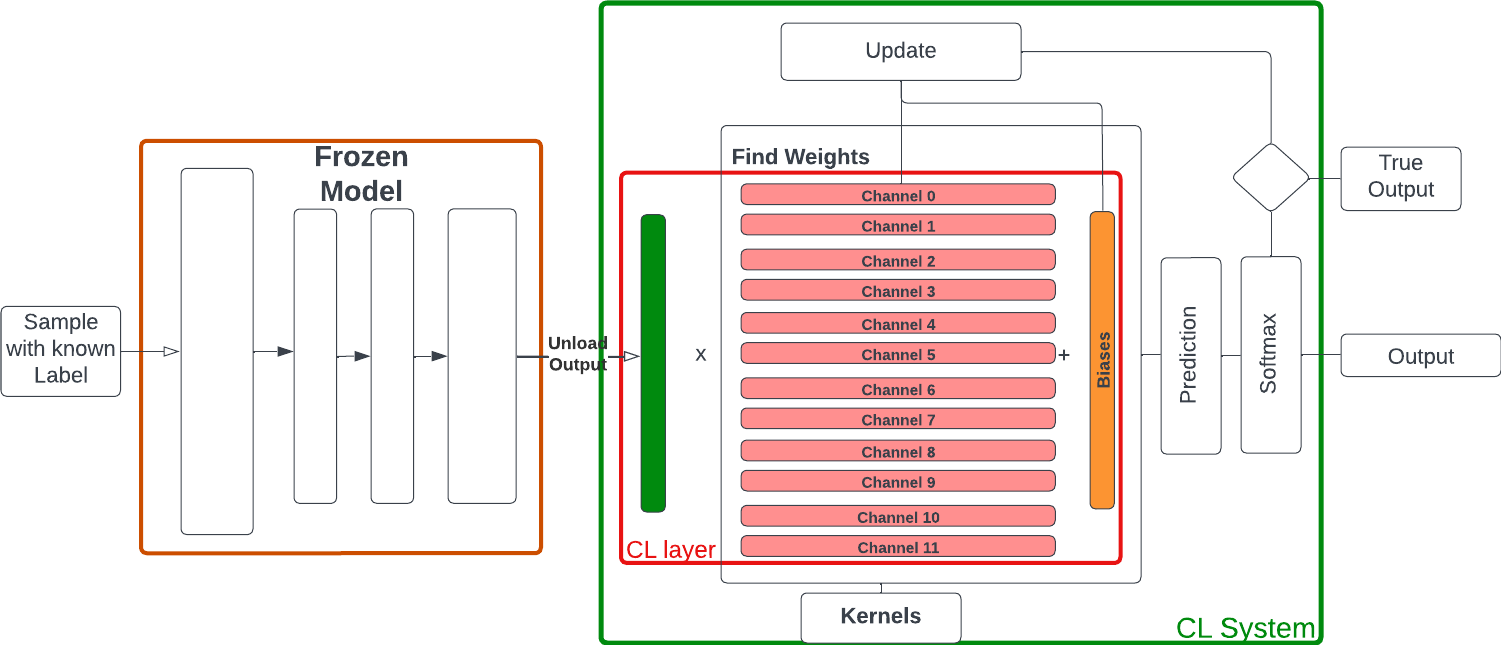
\psfig{file=Images/CL_system.png,width=1\textwidth}}
\caption{Description of TinyOL algorithm on Max78000}
\label{CL_system}
\end{figure}
    



\clearpage
\newpage
\mbox{~}
\clearpage
\newpage

